%!TEX TS-program = pdflatex
\documentclass{article}
\usepackage{CJKutf8}
\usepackage{graphicx}
\usepackage{eepic}
\usepackage{pst-all}
\usepackage{amsmath, amsthm,amsfonts, stmaryrd}
%\usepackage[latin1]{inputenc}
\usepackage[cyr]{aeguill}
%\usepackage[francais]{babel}
\usepackage{listings}
\usepackage{psfrag}
\usepackage{epsfig}

\usepackage{cancel}

%\usepackage{pdftricks}

%\usepackage{bookman}
%\usepackage{helvet}
%\usepackage{newcent}
%\usepackage{aeguill}



\DeclareMathOperator{\sinc}{sinc}


\renewcommand{\v}{\vec} 
\renewcommand{\c}{\times} 
\renewcommand{\o}{\circ}
\renewcommand{\b}{\mathbf} 

\newcommand{\w}{\vec{\omega}} 
\newcommand{\IM}{\vec{\textrm{Im}}} 
\newcommand{\RE}{\textrm{Re}} 

\renewcommand{\wp}{\v{\omega}'}
\newcommand{\dwp}{\dot{\v{\omega}}'}
\newcommand{\wgpp}{\v{\omega}_g''}
\newcommand{\dwgpp}{\dot{\v{\omega}}_g''}
\newcommand{\wg}{\omega_g}
\newcommand{\dwg}{\dot{\omega}_g}
\newcommand{\eg}{\hat{e}_g}

\newcommand{\bq}{\b{q}}
\newcommand{\dbq}{\dot{\b{q}}}
\newcommand{\half}{\frac{1}{2}}

\newcommand{\dG}{\dot{G}}

\newcommand{\ww}{\vec{w}'}

\newcommand{\spaceup}{\phantom {\textrm{\Huge l \normalsize}}}

%\lstset{language=MATLAB}
%\lstset{basicstyle=\footnotesize,frame=single}

%\newenvironment{nom}[nb_arg]{avant}{aprs}

\newcommand{\projectName}{\emph{hydroMEX3 }} %current project name

%MATLAB code listings:
\newcommand{\MATcode}
{
	\lstset{language=MATLAB}
	\lstset{basicstyle=\footnotesize,frame=single,showstringspaces=false}
}
%MATLAB code line:
\newcommand{\MATline}
{
	\lstset{language=MATLAB}
	\lstset{basicstyle=\normalsize,frame=none,showstringspaces=false}
}
%C code listings:
\newcommand{\Ccode}
{
	\lstset{language=C}
	\lstset{basicstyle=\footnotesize,frame=single,showstringspaces=false}
}
%C code line:
\newcommand{\Cline}
{
	\lstset{language=C}
	\lstset{basicstyle=\normalsize,frame=none,showstringspaces=false}
}


\newcommand{\vbeg}{\left( \begin{array}{c} } 
\newcommand{\vend}{ \end{array} \right)} 

\definecolor{cBlue}{rgb}{0.0,0.0,1.0}
\definecolor{cViol}{rgb}{0.4,0.0,0.6}
\definecolor{cRed}{rgb}{0.7,0.0,0.3}
\definecolor{cGreen}{rgb}{0.3,0.5,0.0}
\definecolor{cGrey}{rgb}{0.2,0.2,0.2}
\definecolor{cGreyy}{rgb}{0.5,0.5,0.5}
\definecolor{cBlack}{rgb}{0.0,0.0,0.0}

\newcommand{\Blue}{\color{cBlue}} 
\newcommand{\Viol}{\color{cViol}} 
\newcommand{\Red}{\color{cRed}} 
\newcommand{\Green}{\color{cGreen}} 
\newcommand{\Grey}{\color{cGrey}} 
\newcommand{\Greyy}{\color{cGreyy}} 
\newcommand{\Black}{\color{cBlack}} 

\newcommand{\n}{ \vec n} 
\newcommand{\bn}{\vec{\bar n}} 

\newtheorem{proposition}{Proposition}
%\renewcommand{\epsilon}{\varepsilon}


%\newbox\bwk\edef\tempd#1pt{#1\string p\string t}\tempd\def\nbextr#1pt{#1}
%\def\npts#1{\expandafter\nbextr\the#1\space}
%\def\ttwplink#1#2{\special{ps:1 0 0 setrgbcolor}#2\special{ps:0 0 0 setrgbcolor}\setbox\bwk=\hbox{#2}\special{ps:( linkto #1)\space\npts{\wd\bwk} \npts{\dp\bwk} -\npts{\ht\bwk} true\space Cpos}}
\begin{document}
\begin{CJK*}{UTF8}{gbsn}
%\nocite{{Khalil, Lovera, Wisniewski, CommentsWisniewski, nCube, QFREP, Gros, Gold, Wells, disturbances, Wertz, Wertz2, Gruber, Slotine}}
%\bibliographystyle{unsrt}

%titre etc...:
\title{四元数与动力学}
\author{Basile Graf \\ \texttt{basile.graf@epfl.ch}}
\date{February, 2007}
\maketitle
\thispagestyle{empty}

%%%%%%%%%%%%%%%%%%%%%%%%%%%%%%%%%%%%%%%%%%%%%%%
\subsection*{摘要}
本文简单介绍了四元数及其在动力学中的实际应用。详细介绍了刚体动力学。在附录中,给出了一些更为奇异的关系,这些关系允许编写更为复杂的模型,例如,在非惯性参考系中表示的带有惯性轮的卫星模型。众所周知,四元数相对于欧拉角的一个很好的优点是,除了通常的参数外,它允许完全手工记录相当复杂的动力学。 
%%%%%%%%%%%%%%%%%%%%%%%%%%%%%%%%%%%%%%%%%%%%%%%

\pagebreak

\tableofcontents

%\pagebreak



%\pagebreak

%%%%%%%%%%%%%%%%%%%%%%%%%%%%%%%%%%%%%%%%%%%%%%%

%\section{Referentials}

%Before we derive the dynamics model of the  satellite, we need to introduce the global geometry and introduce some notations. The SwissCube orbit will be almost circular and sun-synchronous (passing near the poles). It can be sketched as follows.

%\begin{center}
%	\psfrag{IRF}[l][c][1][0]{IRF ($\vec{x}_{IRF}$)}
%	\psfrag{ORF}[l][c][1][0]{ORF ($\vec{x}$)}
%	\psfrag{SRF}[l][c][1][0]{\color{cRed}{SRF} ($\vec{x}'$)}
%\psfrag{Orbit}[c][c][0.8][0]{Orbit}
%\psfrag{Earth}[c][c][0.8][0]{Earth}
%	\epsfig{file=figuresIS/referentials.eps, width=7cm}
%\end{center}

%We will deal with three different reference frames. An inertial one, fixed to the Earth, an orbital one (ORF), fixed to the orbit with the positive $x$-direction pointing in the direction of displacement and a positive $z$-direction pointing toward the center of the Earth. The last one is the body-fixed referential (BRF). It coincides with the ORF when the satellite has the desired nominal orientation. \\
%A vector will be denoted by $\v x'$ when expressed in the BRF and by $\v x$ when expressed in the ORF (sometimes also in the IRF, when this is clear from the context). When confusion is possible between IRF and ORF, the notation $\v x_{IRF}$ is used to make the distinction.\\

%Under the term dynamics, we understand the dynamics of the satellite orientation (i.e. attitude) and not the orbital dynamics on which we have no control. The orbital position and speed is considered a pure function of time in this work.\\

%Also, we deal only with the control problem and the state variables are supposed to be known at each time.

%%%%%%%%%%%%%%%%%%%%%%%%%%%%%%%%%%%%%%%%%%%%%%%


%\graphicspath{{SubDocuments/CubsatModel/}}
%\include{SubDocuments/CubsatModel/CubsatModel}

%\graphicspath{{SubDocuments/WheelControllability/}}
%\include{SubDocuments/WheelControllability/WheelControllability}

%\graphicspath{{SubDocuments/CubesatControl/}}
%\include{SubDocuments/CubesatControl/CubesatControl}

%%%%%%%%%%%%%%%%%%%%%%%%%%%%%%%%%%%%%%%%%%%%%%%

%\section{Conclusions}

%During this project, good theoretical and intuitive comprehension of the system has been acquired. \\
%The use of one inertia wheel was seen to be problematic, as it would have to be placed along the only axis that is always controllable with the magnetotorquers in nominal attitude and as it would penalize controllability on the other axes if spinning too fast. \\
%Full magnetic actuation was found to be theoretically feasible, but unfortunately, was also found to be unable to reject the amount of environmental predicted perturbations. \\

%Finally, I would like to thank all the people from the "Laboratoire d'Automatique", in particular my supervisors Philippe Muellhaupt and Sebastien Gros, for their help and valuable advice.
%%%%%%%%%%%%%%%%%%%%%%%%%%%%%%%%%%%%%%%%%%%%%%%%


\pagebreak 

\graphicspath{{SubDocuments/Quaternions/}}
%\documentclass[a4paper]{article}
%\usepackage{graphicx}
%\usepackage{eepic}
%\usepackage{pst-all}
%\usepackage{amsmath, amsthm,amsfonts, stmaryrd}
%%\usepackage[latin1]{inputenc}
%\usepackage[cyr]{aeguill}
%%\usepackage[francais]{babel}
%\usepackage{listings}
%\usepackage{psfrag}
%\usepackage{epsfig}

%%\usepackage{pdftricks}

%%\usepackage{bookman}
%%\usepackage{helvet}
%%\usepackage{newcent}
%%\usepackage{aeguill}

%

%\DeclareMathOperator{\sinc}{sinc}

%
%\renewcommand{\v}{\vec} 
%\renewcommand{\c}{\times} 
%\renewcommand{\o}{\circ}
%\renewcommand{\b}{\mathbf} 

\renewcommand{\w}{\omega} 
%\newcommand{\IM}{\vec{\textrm{Im}}} 
%\newcommand{\RE}{\textrm{Re}} 

%

%%\lstset{language=MATLAB}
%%\lstset{basicstyle=\footnotesize,frame=single}

%%\newenvironment{nom}[nb_arg]{avant}{aprs}

%\newcommand{\projectName}{\emph{hydroMEX3 }} %current project name

%%MATLAB code listings:
%\newcommand{\MATcode}
%{
%	\lstset{language=MATLAB}
%	\lstset{basicstyle=\footnotesize,frame=single,showstringspaces=false}
%}
%%MATLAB code line:
%\newcommand{\MATline}
%{
%	\lstset{language=MATLAB}
%	\lstset{basicstyle=\normalsize,frame=none,showstringspaces=false}
%}
%%C code listings:
%\newcommand{\Ccode}
%{
%	\lstset{language=C}
%	\lstset{basicstyle=\footnotesize,frame=single,showstringspaces=false}
%}
%%C code line:
%\newcommand{\Cline}
%{
%	\lstset{language=C}
%	\lstset{basicstyle=\normalsize,frame=none,showstringspaces=false}
%}

%
%\newcommand{\vbeg}{\left( \begin{array}{c} } 
%\newcommand{\vend}{ \end{array} \right)} 

%\definecolor{cBlue}{rgb}{0.0,0.0,1.0}
%\definecolor{cViol}{rgb}{0.4,0.0,0.6}
%\definecolor{cRed}{rgb}{0.7,0.0,0.3}
%\definecolor{cGreen}{rgb}{0.3,0.5,0.0}
%\definecolor{cGrey}{rgb}{0.2,0.2,0.2}
%\definecolor{cGreyy}{rgb}{0.5,0.5,0.5}
%\definecolor{cBlack}{rgb}{0.0,0.0,0.0}

%\newcommand{\Blue}{\color{cBlue}} 
%\newcommand{\Viol}{\color{cViol}} 
%\newcommand{\Red}{\color{cRed}} 
%\newcommand{\Green}{\color{cGreen}} 
%\newcommand{\Grey}{\color{cGrey}} 
%\newcommand{\Greyy}{\color{cGreyy}} 
%\newcommand{\Black}{\color{cBlack}} 

%
%\begin{document}

%%titre etc...:
%\title{Quaternions}
%\author{
%	Basile Graf 	\vspace{0.1in} \\
%  Ecole Polytechnique Fdrale de Lausanne\\
%  \texttt{basile.graf@epfl.ch}}
%\date{\today}
%\maketitle

%\pagebreak

%

%
%% Rsum:
%\begin{abstract}
%\end{abstract}

%\vspace{30pt}

%
%%Table des matire:
% \tableofcontents

%\newpage

%
%%Sections:
%\section*{Introduction}

%

%\section{}


\section{四元数}
\label{quat}

\subsection{基本原则}

关系方程 \eqref{eq1},以及关联性和分布性都是我们用来推导四元数的基本实际应用的。

\begin{equation}
\fbox{$i^2 = j^2 = k^2 = ijk = -1$}
\label{eq1}
\end{equation}

通过左乘和右乘,在上面的方程中,我们可以写出 


\begin{equation*}
\begin{tabular}{cc}
	\multicolumn{2}{c}{$i\ ijk = -jk = -i$}  \\
	\multicolumn{2}{c}{$ijk\ k = -ij = -k$}  \\
	$j \ jk = -k = ji$  &   $ij \ j = -i = kj$  \\
	$i \ ij = -j = ik$  &   $ji \ i = -j = -ki$ 
\end{tabular}
\end{equation*}

这表明乘积是非交换的(\emph{non commutative}),并给出了基本的乘法规则:

\begin{equation}
\fbox{
\begin{tabular}{cc}
	$ij=k$ & $ji=-k$  \\
	$jk=i$ & $kj=-i$  \\
	$ki=j$ & $ik=-j$  \\
\end{tabular}}
\label{eq3}
\end{equation}



\subsection{符号和定义}

四元数 $q$ 是四个参数的集合,一个实数 $q_0$ 和三个虚数 $q_1i$, $q_2j$, $q_3k$ 以及 $q_1, q_2, q_3 \in  \mathbb{R}$,这可以写为
 
\begin{equation*}
q=q_0+q_1i+q_2j+q_3k .
\end{equation*}

然而,这个符号证明自己是非常不实用的。因此,我们将使用两种不同的符号:

\begin{itemize}
	\item 四元数 $q$ 作为一个实数和一个向量虚数的有序对 \\
			$q = (q_0, \vec{q})  \qquad\qquad   \RE\big\{ q \big\}=q_0  \qquad  \IM\big\{ q \big\}=\vec{q}=(q_1\ q_2\ q_3)^T$
	\item 四个参数的列向量 \\
			$\b{q}=(q_0\ q_1\ q_2\ q_3)^T$
\end{itemize}

$q$ 的共轭 $\bar{q}$ 被定义为

\begin{equation*}
\bar{q} = (q_0, -\vec{q})
\end{equation*}

并且它的范数 (非负实值) 是

\begin{equation*}
|q| = |\b{q}| = \sqrt{q^2_0+q^2_1+q^2_2+q^2_3}.
\end{equation*}

如下一节所述,两个四元数的乘积写成一对,将用符号 $\o$ 标记。


\subsection{四元数乘积}

根据方程 \eqref{eq3}中给出的规则,我们可以写出 $q$ 和 $p$ 的乘积。 


\begin{equation*}
(q_0 + q_1i +q_2j +q_3k) (p_0 + p_1i +p_2j +p_3k) \ =
\label{eq4}
\end{equation*}

\begin{equation*}
\begin{tabular}{ccccccccc}
    & \Greyy{$p_0 q_0$}    &$+$&   \Red{$q_0 p_1 \ i$}   &$+$&   \Red{$q_0 p_2 \ j$}   &$+$&   \Red{$q_0 p_3 \ k$}  & \\
$+$ & \Blue{$q_1 p_0 \ i$} &$+$&   \Green{$q_1 p_1 \ ii$}  &$+$&   $q_1 p_2 \ ij$  &$+$&   $q_1 p_3 \ ik$ & \\
$+$ & \Blue{$q_2 p_0 \ j$} &$+$&   $q_2 p_1 \ ji$  &$+$&   \Green{$q_2 p_2 \ jj$}  &$+$&   $q_2 p_3 \ jk$ & \\
$+$ & \Blue{$q_3 p_0 \ k$} &$+$&   $q_3 p_1 \ ki$  &$+$&   $q_3 p_2 \ kj$  &$+$&   \Green{$q_3 p_3 \ kk$} & $=$ \\
\end{tabular}
\label{eq5}
\end{equation*}




\begin{equation*}
\begin{tabular}{ccccccccc}
    & \Greyy{$p_0 q_0$}   &$-$&   \Green{$q_1 p_1$}   &$-$&   \Green{$q_2 p_2$}    &$-$&   \Green{$q_3 p_3$}   & \\
$+$ & \Blue{$(q_1 p_0$}   &$+$&   \Red{$q_0 p_1$}   &$+$&   $q_2 p_3$    &$-$&   $q_3 p_2)\ i$   & \\
$+$ & \Blue{$(q_2 p_0$}   &$+$&   \Red{$q_0 p_2$}   &$+$&   $q_3 p_1$    &$-$&   $q_1 p_3)\ j$   & \\
$+$ & \Blue{$(q_3 p_0$}   &$+$&   \Red{$q_0 p_3$}   &$+$&   $q_1 p_2$    &$-$&   $q_2 p_1)\ k$   & \\
\end{tabular}
\label{eq6}
\end{equation*}

\begin{equation}
q \circ p = (\Greyy{p_0 q_0} - \Green{\v{p}\cdot\v{q}} , \Red{q_0 \v{p}} + \Blue{p_0 \v{q}} + \Black{\v{q}\c\v{p}}).
\label{eq7}
\end{equation}

从方程 \eqref{eq7} 可以看出

\begin{equation}
q \o \bar{q} = \bar{q} \o q = (|q|^2, \vec{0}) = |q|^2
\label{eqConj}
\end{equation}

并且如果 $q$ 是赋范的 ($|q|=1$)

\begin{equation}
q \o \bar{q} = \bar{q} \o q = (1, \vec{0}) = Id.
\label{eqConjN}
\end{equation}

在方程 \eqref{eq7} 中我们也看到 

\begin{equation}
\overline{q \o p} = \bar{p} \o \bar{q}
\label{eqQoQbar}
\end{equation}

那就是

\begin{equation*}
|q \o p|^2 = (q\o p) \o (\overline{q \o p}) = q\o \underbrace{p \o \bar{p}}_{|p|^2} \o \bar{q} = |p|^2 (q\o \bar{q}) = |q|^2|p|^2
\end{equation*}
\begin{equation}
|q \o p|  = |q||p|.
\label{eqNormProd}
\end{equation}


\subsection{四元数和空间旋转}

首先,注意以下关系

\begin{gather*}
(\vec{u} \c \vec{v}) \c \vec{w} = (\vec{u} \cdot \vec{w}) \vec{v}   -   (\vec{v} \cdot \vec{w}) \vec{u} \\
\sin^2\frac{\varphi}{2} = \frac{1-\cos\varphi}{2}  \qquad    \cos^2\frac{\varphi}{2} = \frac{1+\cos\varphi}{2}.
\end{gather*}

从现在起, $q$ 通常表示一个涉及旋转的赋范四元数 ($|q|=1$) 。现在让我们在四元数 $x$ 的虚部放置一个向量 $\vec{x}\in \mathbb{R}^3$ ,看看它在下面的关系中会发生什么   

\begin{equation*}
x' = \bar{q} \o x \o q  \qquad \qquad   x = (0,\vec{x}) \qquad  q = (q_0, \vec{q}) .  
\end{equation*}

使用方程 \eqref{eq7}

\begin{gather*}
x' = (\vec{q} \cdot \vec{x},\  q_0 \vec{x} - \vec{q} \c \vec{x}) \o q \\
= (  \underbrace{(\vec{q} \cdot \vec{x})q_0 - (q_0 \vec{x} - \vec{q} \c \vec{x}) \cdot \vec{q}}_{\RE\{ x'  \}},\  
\underbrace{(\vec{q} \cdot \vec{x}) \vec{q} + q_0(q_0 \vec{x} - \vec{q} \c \vec{x}) +(q_0 \vec{x} - \vec{q} \c \vec{x}) \c \vec{q}}_{\IM\{  x' \}}  )
\end{gather*}


\begin{align*}
\RE\big\{ x' \big\} &= (\vec{q} \cdot \vec{x})q_0 - q_0(\vec{x} \cdot \vec{q}) - (\vec{q} \c \vec{x}) \cdot \vec{q} = 0 \\
                    &\Rightarrow \ x' = (0,\vec{x}'), \\
\IM\big\{ x' \big\} &= \vec{x}' \\
										&= (\vec{q} \cdot \vec{x}) \vec{q} + q_0^2\vec{x} - q_0(\vec{q}\c\vec{x}) + q_0(\vec{x}\c\vec{q}) - (\vec{q}\c\vec{x}) \c\vec{q} \\
                    &= (\vec{q} \cdot \vec{x}) \vec{q} + q_0^2\vec{x} + 2 q_0(\vec{x}\c\vec{q}) - (\vec{q}\c\vec{x}) \c\vec{q} \\
    &= (\vec{q} \cdot \vec{x}) \vec{q} + q_0^2\vec{x} + 2 q_0(\vec{x}\c\vec{q}) - (\vec{q}\cdot\vec{q})\vec{x} + (\vec{x}\cdot\vec{q})\vec{q} \\
    &= 2(\vec{q} \cdot \vec{x}) \vec{q} + q_0^2\vec{x} + 2 q_0(\vec{x}\c\vec{q}) - (\vec{q}\cdot\vec{q})\vec{x}.
\end{align*}


一个有效的赋范四元数 ($|q|=\sqrt{(q_0^2+q_1^2+q_2^2+q_3^2)}=1$) 将会

\begin{equation*}
q = (q_0, \vec{q}) = (\cos\frac{\varphi}{2},\ \sin\frac{\varphi}{2}\vec{n}) \qquad \qquad |\vec{n}|=1.
\end{equation*}

在这种情况下, $\vec{x}'$ 变成 

\begin{align*}
\vec{x}'  &=  
2 \sin^2\frac{\varphi}{2} (\vec{n}\cdot\vec{x})\vec{n} + \cos^2\frac{\varphi}{2} \vec{x} + 2 \cos\frac{\varphi}{2} \sin\frac{\varphi}{2} (\vec{x}\c\vec{n}) - \sin^2\frac{\varphi}{2} \vec{x} \\
         &= (1-\cos\varphi)(\vec{n}\cdot\vec{x}) \vec{n}  + \cos\varphi\ \vec{x} + \sin\varphi\ (\vec{x}\c\vec{n}).
\end{align*}

最后一个关系是用一个角度 $\varphi$ 绕一个赋范轴矢量 $\vec{n}$ 的旋转公式,如下图所示:

\begin{figure}
\begin{center}
\psfrag{0}[l][c][1][0]{$0$}
\psfrag{n}[l][c][1][0]{$\vec{n}$}
\psfrag{xnn}[l][c][1][29]{$(\vec{x}\cdot\vec{n})\vec{n}$}
\psfrag{x}[l][c][1][0]{$\vec{x}$}
\psfrag{xp}[l][c][1][0]{$\vec{x}'$}
\psfrag{v1}[l][c][1][0]{$\vec{v}_1$}
\psfrag{v2}[l][c][1][0]{$\vec{v}_2$}
\psfrag{v3}[l][c][1][0]{$\vec{v}_3$}
\psfrag{phi}[l][c][1][0]{$\varphi$}
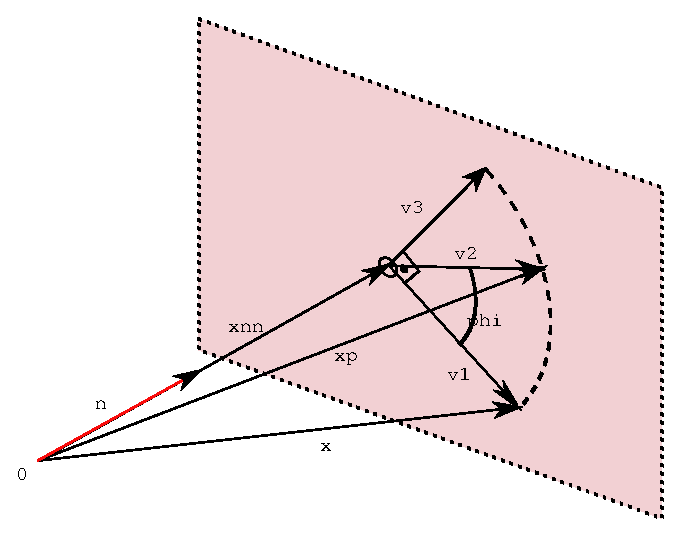
\epsfig{file=figures/rotation.eps, width=8cm}
\end{center}
\end{figure}


\begin{align*}
\vec{v}_2 &= \cos\varphi\ \vec{v}_1 + \sin\varphi\ \vec{v}_3 \\
\vec{v}_1 &= \vec{x} - (\vec{x}\cdot\vec{n})\vec{n} \\
\vec{v}_3 &= \vec{v}_1 \c \vec{n}  \\
          &= (\vec{x} - (\vec{x}\cdot\vec{n})\vec{n}) \c \vec{n} \\
          &= (\vec{x}\c\vec{n}) - (\vec{x}\cdot\vec{n})\underbrace{\vec{n}\c\vec{n}}_{\vec{0}} \\
\Rightarrow\ \vec{v}_2 &= \cos\varphi\ (\vec{x} - (\vec{x}\cdot\vec{n})\vec{n}) + \sin\varphi\ (\vec{x}\c\vec{n}) \phantom{\underbrace{1}_{\vec{1}}}\\
\vec{x}'  &= (\vec{x}\cdot\vec{n})\vec{n} + \vec{v}_2 \\
          &= (\vec{x}\cdot\vec{n})\vec{n} + \cos\varphi\ (\vec{x} - (\vec{x}\cdot\vec{n})\vec{n}) + \sin\varphi\ (\vec{x}\c\vec{n}) \\
          &= (1-\cos\varphi)(\vec{n}\cdot\vec{x}) \vec{n}  + \cos\varphi\ \vec{x} + \sin\varphi\ (\vec{x}\c\vec{n}).
\end{align*}

而且

\begin{gather*}
x' = \bar{q} \o x \o q \\
q \o x' \o \bar{q} = \underbrace{q\o\bar{q}}_{(1,\vec{0})} \o x \o \underbrace{q\o\bar{q}}_{(1,\vec{0})}.
\end{gather*}

因此我们得到了旋转及其逆的关系

\begin{equation}
\fbox{$x' = \bar{q} \o x \o q \\   \qquad  x = q \o x' \o \bar{q}$}.
\end{equation}



\subsection{四元数和旋转速度}

我们现在将推导旋转速度矢量和四元数时间导数之间的关系。 $\vec{x}'$ 是任意恒定矢量,位于机体参考坐标系(\emph{body (rotating) reference frame})中,并且 $\vec{x}$ 是在固定参考坐标系(\emph{fixed reference frame})中的同一个矢量。如前所述,两个矢量都可以与

\begin{equation*}
\begin{tabular}{ccc}
$x = q \o x' \o \bar{q}$ &  & $x' = \bar{q} \o x \o q$.
\end{tabular}
\label{eq8}
\end{equation*}

将时间导数应用于 $x=(0,\vec{x})$,以及 $x'=(0,\vec{x}')$ 和 $\dot{\vec{x}}'=\v{0}$,我们得到

\begin{gather*}
\dot{x} = \dot{q} \o x' \o \bar{q}  +  q \o x' \o \dot{\bar{q}}  \\
\dot{x} = \dot{q} \o \bar{q} \o x \o \underbrace{q \o \bar{q}}_{Id}  +  \underbrace{q \o \bar{q}}_{Id} \o x \o q \o \dot{\bar{q}}
\end{gather*}
\begin{equation}
\dot{x} = \dot{q} \o \bar{q} \o x  +   x \o q \o \dot{\bar{q}}  
\label{eq9.3}
\end{equation}

并且从方程 \eqref{eq7}

\begin{gather*}
\dot{q} \o \bar{q} = ( \underbrace{\dot{q_0}q_0 + \dot{\v{q}}\cdot\v{q}}_{\varoast}, -\dot{q_0}\v{q} + q_0\dot{\v{q}} - \dot{\v{q}} \c \v{q}) \\
\varoast = q_0\dot{q_0} + q_1\dot{q_1} + q_2\dot{q_2} + q_3\dot{q_3} = \b{q} \cdot \dot{\b{q}} = 0
\end{gather*}

因为 $|\b{q}|=1$。那就是

\begin{equation}
\dot{q} \o \bar{q} = (0,\v{\nu})  \qquad \textrm{and similarly} \qquad \bar{q} \o \dot{q} = (0,\v{-\nu}). 
\label{eq10}
\end{equation}


\subsubsection{固定参考系中的转速 $\w$}
从方程 \eqref{eq9.3} 和 \eqref{eq10} 并且使用 \eqref{eq7} 我们有

\begin{align*}
\dot{x} & = (0,\v{\nu}) \o x - x \o (0,\v{-\nu})  \\
\dot{\vec{x}} & = \vec{\nu} \c \vec{x} - \vec{x} \c \vec{\nu} = 2 \vec{\nu} \c \vec{x}
\end{align*}
并且从方程 \eqref{eqNormProd} 
\begin{equation*}
|\dot{\vec{x}}|=|2\vec{\nu}||\vec{x}|  \qquad \Rightarrow \qquad    \vec{\nu} \bot \vec{x}
\end{equation*}


如果 $\vec{x}$ 经历纯旋转,我们知道这个

\begin{equation*}
\dot{\vec{x}} = \vec{\w} \c \vec{x}    \qquad \textrm{and} \qquad   \vec{\w} \bot \vec{x}
\end{equation*}

因此


\begin{equation}
\fbox{ $\w = (0,\vec{\w}) = 2(0,\vec{\nu}) = 2 \dot{q} \o \bar{q} $}.
\end{equation}

并且右乘以 $q$

\begin{equation*}
\w \o q= 2 \dot{q} \o \underbrace{\bar{q} \o q}_{Id} \ \  \Rightarrow \ \  \w \o q = 2 \dot{q}
\end{equation*}

\begin{equation}
\fbox{$ \dot{q} = \frac{1}{2} \w \o q $}.
\end{equation}




\subsubsection{机体参考系中的转速 $\w'$}

\begin{align*}
             \w'      & = \bar{q} \o \w \o q    \qquad \textrm{with} \qquad    \w = 2 \dot{q} \o \bar{q} \\
\Rightarrow  \ \ \w'  & = 2 \bar{q} \o \dot{q} \o \underbrace{\bar{q} \o q}_{Id}
\end{align*}

\begin{equation}
\fbox{ $\w' = 2 \bar{q} \o \dot{q} $}.
\end{equation}

并且左乘以 $q$

\begin{equation*}
q \o \w' = 2 \underbrace{q \o \bar{q}}_{Id} \o \dot{q} = 2 \dot{q}
\end{equation*}

\begin{equation}
\fbox{$ \dot{q} = \frac{1}{2} q \o \w' $}.
\end{equation}




\subsubsection{矩阵乘积表示的 $\w$}
\label{secMat1}

从

\begin{equation*}
\w = 2 \dot{q} \o \bar{q} 
\end{equation*}

并且使用方程 \eqref{eq7}

\begin{align*}
\vec{\w} &= \IM\big\{{2 \dot{q} \o \bar{q}} \big\} = 2(\Red{-\dot{q_0}\vec{q}} \Blue{ + q_0\dot{\vec{q}}} \Black{- \dot{\vec{q}} \c \vec{q})} \\
         &= 2 \underbrace{\left( \begin{array}{cccc}
\Red{-q_1} &  \Blue{q_0} & -q_3 & q_2 \\
\Red{-q_2} &  q_3 & \Blue{q_0}  & -q_1 \\
\Red{-q_3} & -q_2 & q_1  & \Blue{q_0} \\
\end{array} \right)}_{E} \left( \begin{array}{c}
\dot{q_0} \\
\dot{q_1} \\
\dot{q_2} \\
\dot{q_3} \\
\end{array} \right)
\end{align*}

\begin{equation*}
\vec{\w} = 2E\dot{\b{q}} .
\end{equation*}

更改符号并反转交叉积可以制造另一个标识

\begin{equation*}
\vec{\w} = -2(-q_0\dot{\vec{q}} + \dot{q_0}\vec{q} - \vec{q} \c \dot{\vec{q}}) 
\end{equation*}

\begin{equation*}
\vec{\w} = -2\dot{E}\b{q} .
\end{equation*}

因此,固定参考系(\emph{fixed reference})中的转速矢量可以写为

\begin{equation}
\fbox{$ \vec{\w} = 2E\dot{\b{q}} = -2\dot{E}\b{q} $} .
\end{equation}


并且从

\begin{equation*}
\dot{q} = \frac{1}{2} \w \o q     \qquad \qquad  \w = (0,\vec{\w}) \ \Rightarrow \ \w_0=0
\end{equation*}

同样,我们也可以发现

\begin{equation*}
\dot{\b{q}} = \frac{1}{2} \left( \begin{array}{c}
(-\vec{\w} \cdot \vec{q})\\
(q_0\vec{\w} + \vec{\w} \c \vec{q})
\end{array} \right) = \frac{1}{2} E^T\vec{\w}
\end{equation*}

\begin{equation}
\fbox{$ \dot{\b{q}} = \frac{1}{2} E^T\vec{\w} $} .
\label{eq_dotq_w}
\end{equation}


\subsubsection{矩阵乘积表示的 $\w'$}
\label{secMat2}

从

\begin{equation*}
\w' = 2 \bar{q} \o \dot{q} 
\end{equation*}

并且使用方程 \eqref{eq7}

\begin{align*}
\vec{\w'} &= \IM\big\{{2 \bar{q} \o \dot{q}} \big\} = 2(\Blue{q_0\dot{\vec{q}}} \Red{ - \dot{q_0}\vec{q}} \Black{- \vec{q} \c \dot{\vec{q}})} \\
         &= 2 \underbrace{\left( \begin{array}{cccc}
\Red{-q_1} &  \Blue{q_0} & q_3 & -q_2 \\
\Red{-q_2} & -q_3 & \Blue{q_0}  & q_1 \\
\Red{-q_3} & q_2 & -q_1  & \Blue{q_0} \\
\end{array} \right)}_{G} \left( \begin{array}{c}
\dot{q_0} \\
\dot{q_1} \\
\dot{q_2} \\
\dot{q_3} \\
\end{array} \right)
\end{align*}

\begin{equation*}
\vec{\w'} = 2G\dot{\b{q}} .
\end{equation*}

改变符号并反转交叉积可以制造另一个标识

\begin{equation*}
\vec{\w'} = -2(\dot{q_0}\vec{q} - q_0\dot{\vec{q}} - \dot{\vec{q}} \c \vec{q}) 
\end{equation*}

\begin{equation*}
\vec{\w'} = -2\dot{G}\b{q} .
\end{equation*}

所以机体参考系(\emph{body reference})中的旋转速度矢量可以写为

\begin{equation}
\fbox{$ \vec{\w'} = 2G\dot{\b{q}} = -2\dot{G}\b{q} $} .
\label{eqGq}
\end{equation}



并且从

\begin{equation*}
\dot{q} = \frac{1}{2} q \o \w'     \qquad \qquad  \w' = (0,\vec{\w'}) \ \Rightarrow \ \w'_0=0
\end{equation*}

同样,我们也可以发现

\begin{equation*}
\dot{\b{q}} = \frac{1}{2} \left( \begin{array}{c}
(-\vec{q} \cdot \vec{\w'})\\
(q_0\vec{\w'} + \vec{q} \c \vec{\w'})
\end{array} \right) = \frac{1}{2} G^T\vec{\w'}
\end{equation*}

\begin{equation}
\fbox{$ \dot{\b{q}} = \frac{1}{2} G^T\vec{\w'} $} .
\label{eqqdot}
\end{equation}




\subsubsection{旋转矩阵 $R$}

我们已经有

\begin{minipage}[left]{0.49 \textwidth}
	\begin{gather*}
	   	 \vec{\w} = 2E\dot{\b{q}} = -2\dot{E}\b{q}  \\
		\dot{\b{q}} = \frac{1}{2} E^T\vec{\w}
	\end{gather*}
\end{minipage}
\begin{minipage}[right]{0.49 \textwidth}
	\begin{gather*}
	   	 \vec{\w'} = 2G\dot{\b{q}} = -2\dot{G}\b{q}  \\
		\dot{\b{q}} = \frac{1}{2} G^T\vec{\w'}
	\end{gather*}
\end{minipage}


所以我们可以写

\begin{minipage}[left]{0.49 \textwidth}
	\begin{align*}
		\vec{\w} &= 2E\dot{\b{q}}   \\
		         &= 2E(\frac{1}{2} E^T\vec{\w})   \\
		         &= EE^T \vec{\w}   \\
		&\Rightarrow \ \fbox{$EE^T = Id$} .
	\end{align*}
\end{minipage}
\begin{minipage}[right]{0.49 \textwidth}
	\begin{align*}
		\vec{\w'} &= 2G\dot{\b{q}}   \\
		         &= 2G(\frac{1}{2} G^T\vec{\w'})   \\
		         &= GG^T \vec{\w'}   \\
		&\Rightarrow \ \fbox{$GG^T = Id$} .
	\end{align*}
\end{minipage} \\


并且两边混合

\begin{gather*}
	\vec{\w'} = 2G\dot{\b{q}} = 2G(\frac{1}{2} E^T\vec{\w}) = GE^T \vec{\w} \\
	\vec{\w} = 2E\dot{\b{q}} = 2E(\frac{1}{2} G^T\vec{\w'}) = EG^T \vec{\w'} .
\end{gather*}


我们现在应该记得,$\v{\w}$ 是在固定参考系(\emph{fixed reference frame})中的矢量,并且 $\v{\w}'$ 是同一个矢量位于机体参考系(\emph{body reference frame}),就是说 $\vec{\w} = R \vec{\w'}$。通过与前两个结果的比较,我们发现

\begin{equation}
\fbox{$ R = EG^T $} \qquad \textrm{and} \qquad \fbox{$R^{-1}=R^T=GE^T $} .
\label{eqRot}
\end{equation}








\subsubsection{$E\b{p}$ 和 $G\b{p}$}

从在第 \ref{secMat1} 和 \ref{secMat2} 节制造的标识可以看出, $E$ 和 $G$ 与任何四元数 $\b{p}$ 的乘积的一般含义是

\begin{equation}
E\b{p} = \IM\big\{{p \o \bar{q}}\big\}    \qquad \qquad    G\b{p} = \IM\big\{{\bar{q} \o p} \big\} .
\label{eqEpGp}
\end{equation}

并且从

\begin{equation*}
q \o \bar{q} = \bar{q} \o q = (|q|, \vec{0}) = (1,\vec{0})    
\end{equation*}

接下来是

\begin{equation*}
\fbox{$E\b{q} = \vec{0}$}    \qquad \qquad    \fbox{$G\b{q} = \vec{0}$} .
\end{equation*}






\subsubsection{最后一个关系}

对于任何 $\vec{v}$ ,由于关联性

\begin{align*}
\underbrace{(0,\vec{\w'})}_{2 \bar{q} \o \dot{q}} \o (0,\vec{v})  &=  (-\vec{\w'}\cdot\vec{v} , \vec{\w'}\c \vec{v}) \\
           &= 2 \bar{q} \o \dot{q} \o v \\
           &=  2(\Greyy{q_0\dot{q_0}} \Green{+\vec{q} \cdot \dot{\vec{q}}},  \Blue{q_0\dot{\vec{q}}} \Red{ - \dot{q_0}\vec{q}} \Black{- \vec{q} \c \dot{\vec{q}})} \o v =
2 \bar{q} \o (\Greyy{\dot{q_0}v_0} \Green{-\dot{\vec{q}} \cdot \vec{v}},  \Blue{\dot{q_0}\vec{v}} \Red{ + v_0\dot{\vec{q}}} 
\Black{+ \dot{\vec{q}} \c \vec{v}}) \\
         &\equiv 2 \left( \begin{array}{cccc}
\Greyy{q_0} & \Green{q_1} & \Green{q_2} & \Green{q_3} \\
\hline
\Red{-q_1} &  \Blue{q_0} & q_3 & -q_2 \\
\Red{-q_2} & -q_3 & \Blue{q_0}  & q_1 \\
\Red{-q_3} & q_2 & -q_1  & \Blue{q_0} \\
\end{array} \right) 
\left( \begin{array}{c|cccc}
\Greyy{\dot{ q_0}} &  \Green{\dot{-q_1}} & \Green{\dot{-q_2}} & \Green{\dot{-q_3}}\\
\Red{\dot{ q_1}} &  \Blue{\dot{ q_0}} & \dot{-q_3} & \dot{ q_2}\\
\Red{\dot{ q_2}} &  \dot{ q_3} & \Blue{\dot{ q_0}} & \dot{-q_1}\\
\Red{\dot{ q_3}} &  \dot{-q_2} & \dot{ q_1} & \Blue{\dot{ q_0}}\\
\end{array} \right) 
\left( \begin{array}{c}
0 \\
\hline
v_1 \\
v_2 \\
v_3 \\
\end{array} \right) \\
         &= 2 \left( \begin{array}{c}
         \b{q}^T \\
         G  \\
         \end{array} \right) 
         \bigg(\begin{array}{cc}
         \dot{\b{q}} & \dot{G}^T \\
         \end{array} \bigg) 
         \bigg(\begin{array}{c}
         0 \\
         \vec{v} \\
         \end{array} \bigg) = 
         \bigg(\begin{array}{c}
         -\vec{\w'}\cdot\vec{v} \\
         \vec{\w'}\c \vec{v}\\
         \end{array} \bigg)\\
     &\Rightarrow \ 2G\dot{G}^T\vec{v}=\Omega' \vec{v} = \vec{\w'} \c \vec{v} .
\end{align*}

与方程 \eqref{eqGq}相比,我们的结论是

\begin{equation}
\fbox{$ \Omega'= 2G\dot{G}^T = -2\dot{G}G^T \qquad \textrm{and} \qquad  \Omega' \vec{v} = \vec{\w'} \c \vec{v} $} .
\label{eqCross}
\end{equation}






\subsubsection{关系总结}

下表总结了已开发的关系。 $q$ 始终是赋范四元数,即 $q_0^2+q_1^2+q_2^2+q_3^2=1$。 \\
\begin{center}
\begin{tabular}{| p{0.249\textwidth} | p{0.249\textwidth} | p{0.249\textwidth} | p{0.249\textwidth} |}
\hline
\multicolumn{2}{|c|}{四元数表示法}&
\multicolumn{2}{|c|}{矩阵表示法}\\
\hline
\multicolumn{1}{|c|}{\emph{固定参考系}} &
\multicolumn{1}{|c|}{\emph{机体参考系}} &
\multicolumn{1}{|c|}{\emph{固定参考系}} &
\multicolumn{1}{|c|}{\emph{机体参考系}} \\
\hline
$x = q \o x' \o \bar{q}     \phantom{\Bigg(}$  &
$x' = \bar{q} \o x \o q$  &
\begin{tabular}{l}
	$\vec{x}=R\vec{x}'$ \\
	$R=EG^T$
\end{tabular}&
\begin{tabular}{l}
	$\vec{x}'=R^T\vec{x}$  \\
	$R^T=R^{-1}=GE^T$ 
\end{tabular}\\
\hline
$\w=(0,\vec{\w})=2\dot{q}\o\bar{q}     \phantom{\Bigg(}$  &
$\w'=(0,\vec{\w}')=2\bar{q}\o\dot{q}$  &
$\vec{\w}=2E\dot{\b{q}}=-2\dot{E}\b{q}$  &
$\vec{\w}'=2G\dot{\b{q}}=-2\dot{G}\b{q}$ \\
\hline
$\dot{q}=\frac{1}{2}\w \o q     \phantom{\Bigg(}$  &
$\dot{q}=\frac{1}{2} q \o \w'$  &
$\dot{\b{q}}=\frac{1}{2}E^T\vec{\w}$  &
$\dot{\b{q}}=\frac{1}{2}G^T\vec{\w}'$  \\
\hline
&
&
$EE^T=Id     \phantom{\Bigg(}$  &
$GG^T=Id$  \\
\hline
\multicolumn{2}{|c|}{$q\o\bar{q} = \bar{q}\o q = (|q|,\vec{0})     \phantom{\Bigg(}$} &
$E\b{q}=\vec{0}$ &
$G\b{q}=\vec{0}$ \\
\hline
$     \phantom{\Bigg(}$   &
\begin{tabular}{l}
	$(0,\vec{\w}) \o (0,\vec{v}) = $ \\
	$(-\vec{\w'}\cdot\vec{v},\vec{\w'}\c\vec{v})$ 
\end{tabular}&
&
\begin{tabular}{l}
	$\Omega' = 2G\dot{G}^T$ \\
	$\ \ \ \  = -2\dot{G}G^T$  \\
	$\Omega'\vec{v} = \vec{\w'}\c\vec{v}$ 
\end{tabular}\\
\hline
\end{tabular}
\end{center}

\begin{equation*}
E =
\left( \begin{array}{cccc}
-q_1 &  q_0 & -q_3 & q_2  \\
-q_2 &  q_3 & q_0  & -q_1 \\
-q_3 & -q_2 & q_1  & q_0  \\
\end{array} \right)
\qquad \qquad
G = 
\left( \begin{array}{cccc}
-q_1 &  q_0 & q_3 & -q_2 \\
-q_2 & -q_3 & q_0  & q_1 \\
-q_3 & q_2 & -q_1  & q_0 \\
\end{array} \right)
\end{equation*}







\subsection{刚体旋转动力学}
\label{quat_rigid_dyn_IN}

我们现在来看看一个自由旋转的刚体的动力学,这个刚体上应用了动量 $\v T'$ 。不讨论物体的平移 (它可以与旋转动力学分离,而且相当容易)。我们还将考虑一个无势系统,这样拉格朗日方程只恢复到转动动能

\begin{equation}
L=E_{\textrm{rot}}=\frac{1}{2}\vec{\w}'^TJ\vec{\w}'.
\end{equation}

使用四元数 $\b{q}$ 作为坐标,且有约束 $C=\b{q}^T\b{q}=1$,拉格朗日动力学给出

\begin{equation}
\frac{d}{dt}\frac{\partial L}{\partial \dot{\b{q}}} - \frac{\partial L}{\partial \b{q}} = \b{F_q} + {\lambda} \frac{\partial C}{\partial \b{q}}.
\label{eqLDyn}
\end{equation}

$\b{F_q}$ 是广义力的 4-vector,稍后将用施加的扭矩表示。 $\b{\lambda}$ 是用来满足约束 $C$ 的拉格朗日乘子。

\subsubsection{$L$ 的导数}

注意以下提醒

\begin{center}
\begin{tabular}{c}
$\frac{\displaystyle \partial A\b{x}}{\displaystyle \partial \b{x}} = A      \phantom{\Bigg(}$ \\
$\frac{\displaystyle \partial \b{a}^T\b{x}}{\displaystyle \partial \b{x}} = \frac{\displaystyle \partial \b{x}^T\b{a}}{\displaystyle \partial \b{x}} = \b{a}$ \\
$\frac{\displaystyle \partial \b{x}^T A\b{x}}{\displaystyle \partial \b{x}} = (A^T +A)\b{x} \stackrel{\textrm{if }A=A^T}{=} 2A\b{x}     \phantom{\Big(}$ \\
(写成列向量)\\
$(AB)^T=B^TA^T \ .  \phantom{\Bigg(}$\\
\end{tabular}
\end{center}

我们现在导出方程 \eqref{eqLDyn} 左边的每一项。首先,让我们用两种不同的方法重写 $L$ 。
 

\begin{equation*}
L=\frac{1}{2}\vec{\w}'^TJ\vec{\w}' = 2(G\dot{\b{q}})^T J (G\dot{\b{q}}) = 2 (\dot{G}\b{q})^T J (\dot{G}\b{q})
\end{equation*}

并且在围绕 $J$ 分组

\begin{equation*}
L=\frac{1}{2}\vec{\w}'^TJ\vec{\w}' = 2\dot{\b{q}}^T (G^T J G) \dot{\b{q}} = 2 \b{q}^T (\dot{G}^T J \dot{G}) \b{q}.
\end{equation*}

因为 $J$ 是对称的, $(G^T J G)$ 和 $(\dot{G}^T J \dot{G})$ 也是对称的。所以我们有

\begin{equation}
\frac{\partial L}{\partial \b{q}} = 4 \dot{G}^T J \dot{G} \b{q} = 2 \dot{G}^T J \underbrace{(2\dot{G}\b{q})}_{-\vec{\w}'} =
-2 \dot{G}^T J \vec{\w}',
\end{equation}

\begin{equation*}
\frac{\partial L}{\partial \dot{\b{q}}} = 4 G^T J G \dot{\b{q}} = 2 G^T J \underbrace{(2G\dot{\b{q}})}_{\vec{\w}'} =
2 G^T J \vec{\w}'
\end{equation*}

并且

\begin{equation}
\frac{d}{dt} \frac{\partial L}{\partial \dot{\b{q}}} = \frac{d}{dt} (2 G^T J \vec{\w}') = 2 \dot{G}^T J \vec{\w}' + 2 G^T J \dot{\vec{\w}}'.
\end{equation}


\subsubsection{广义力}

找到相对于坐标 $\b{c}$ 的广义力 $\b{F_c}$ 的一种方法就是识别它于方程 

\begin{equation*}
\delta W = \b{F_c} \cdot \delta \b{c} .
\end{equation*}

(一个简单的例子是粒子的纯平移 $\delta \vec{x}$ ,在其上施加一个外力 $\vec{F}$ 。因此,做功是 $\delta W = \b{F}_{\vec{x}} \cdot \delta \vec{x} = \vec{F} \cdot \delta \vec{x}$。因此,在这种情况下,广义力 $\b{F}_{\vec{x}}$ 是简单的 $\vec{F}$ 。) \\

对于一个刚体,施加一个扭矩 $\vec{T}'$,它围绕着轴 $\vec{n}$ ,旋转一个角度 $\delta \varphi$ ,做功可以写为

\begin{equation}
\delta W = (\vec{n} \cdot \vec{T}') \delta \varphi  \qquad \qquad   |\vec{n}|=1.
\label{eqWTfi}
\end{equation}

这种微小的姿态变化可以在一边表示为坐标四元数 $q$ 的微小变化 $\delta q$ ,在另一边表示为从 $q$ 表示的当前姿态(即,组合)操作的旋转四元数 $q_\delta$ 。那就是

\begin{gather*}
q + \delta q = q \o q_\delta    \\
|q|=1 \qquad   |q_\delta|=1  \qquad    |\delta q| \ll 1.
\end{gather*}

我们不需要考虑变量 $\delta q$ 必须保持 $q$的范数这一事实,因为在拉格朗日公式(Lagrange formulation)中引入一个约束,它将自动得到满足。\\

这一边我们可以写

\begin{gather*}
q + \delta q = q \o q_\delta    \\
\underbrace{\bar{q} \o q}_{(1,\vec{0})} + \bar{q} \o \delta q = \underbrace{\underbrace{\bar{q} \o q}_{(1,\vec{0})} \o q_\delta}_{q_\delta}    
\end{gather*}

\begin{equation}
\Rightarrow \ q_\delta = (1,\vec{0}) + \bar{q} \o \delta q.
\label{eq_qdelta}
\end{equation}

在另一边

\begin{equation*}
q_\delta = (\cos{\frac{\delta \varphi}{2}},\  \sin{\frac{\delta \varphi}{2}}\ \vec{n}).
\end{equation*}

考虑虚数部分

\begin{gather*}
\IM\big\{ q_\delta \big\} = \IM\big\{ \bar{q} \o \delta q \big\} = \sin{\frac{\delta \varphi}{2}}\ \vec{n} \approx  \frac{\delta \varphi}{2}\ \vec{n}
\end{gather*}

与方程 \eqref{eqWTfi} 相比

\begin{equation*}
\Rightarrow \ \delta W = 2 \  \IM\big\{ \bar{q} \o \delta q \big\} \cdot \vec{T}'
\end{equation*}


并且从方程 \eqref{eqEpGp}

\begin{gather*}
\IM\big\{ \bar{q} \o \delta q \big\} = G \b{\delta q} \\
\Rightarrow \ \delta W = 2(G \b{\delta q}) \cdot \vec{T}' = 2 \vec{T}'^T (G \b{\delta q})  = 2(G^T \vec{T}')^T \b{\delta q} = \underbrace{2(G^T \vec{T}')}_{\b{F_q}} \cdot \b{\delta q}
\end{gather*}

\begin{equation}
\Rightarrow \ \fbox{$ \b{F_q} = 2G^T \vec{T}'$}.
\label{eqForce}
\end{equation}


\subsubsection{动力学}
\label{quat_rigid_dyn_IN_3}

我们现在有一切可以写动力学的知识

\begin{gather*}
\frac{d}{dt}\frac{\partial L}{\partial \dot{\b{q}}} - \frac{\partial L}{\partial \b{q}} = \b{F_q} + \lambda \frac{\partial C}{\partial \b{q}} \\
4 \dot{G}^T J \vec{\w}' + 2 G^T J \dot{\vec{\w}}' = 2G^T \vec{T}' + \lambda \b{q}. \\
\end{gather*}

左乘以 $G$

\begin{gather*}
\underbrace{4 G \dot{G}^T}_{2\Omega'} J \vec{\w}' + 2 \underbrace{GG^T}_{Id} J \dot{\vec{\w}}' = 2 \underbrace{GG^T}_{Id} \vec{T}' + \lambda \underbrace{G \b{q}}_{\vec{0}} \\
\Omega' J \vec{\w}' +  J \dot{\vec{\w}}' =  \vec{T}' \\
\vec{\w}' \c J \vec{\w}' +  J \dot{\vec{\w}}' =  \vec{T}' \\
J \dot{\vec{\w}}' =  \vec{T}' - \vec{\w}' \c J \vec{\w}'.  
\end{gather*}

最后一个关系就是旋转机体的欧拉运动方程。与方程 \eqref{eqqdot} 一起,我们得到了完全动力学

\begin{equation}
\begin{tabular}{|rcl|}
	\hline
	$\dot{\vec{\w}}'$ & $=$ & $J^{-1} \vec{T}' - J^{-1} (\vec{\w}' \c J \vec{\w}')   \phantom{\Big(}$ \\
	$\dot{\b{q}}$     & $=$ & $\frac{1}{2} G^T\vec{\w}'.   \phantom{\Big(}$ \\
	\hline
\end{tabular}
\label{rigid_euler_IN}
\end{equation}


%%\IM\big\{{2 \bar{q} \o \dot{q}} \big\}

%
%%Bibliographie:
%\begin{thebibliography}{9}

%\bibitem{QFREP}
%	Quaternion, Finite Rotation and Euler Parameters\\
%	Arend L. Schwab \\
%	\emph{http://tam.cornell.edu/\~{}als93/quaternion.pdf}
%	
%\bibitem{Gros}
%	Quaternion based dynamics - Single Turbine Aircraft - Lagrange and Hamiltonian approaches \\
%	S. Gros\\
%	LA, EPFL.
%		
%\bibitem{Gold}
%	Classical Mechanics \\
%	Herbert Goldstein.
%	
%\bibitem{Wells}
%	Lagrangian Dynamics \\
%	Dare A. Wells \\
%	Schaum's Outline Series.
%	
%%\bibitem{Khalil}
%%	Nonlinear Systems \\
%%	Third Edition \\
%%	Hassan K. Khalil \\
%%	Prentice Hall.
%	
%	

%%	\bibitem{lamport94}
%%	  Leslie Lamport,
%%	  \emph{\LaTeX: A Document Preparation System}.
%%	  Addison Wesley, Massachusetts,
%%	  2nd Edition,
%%	  1994.

%%rajouter: bouquin de Papa (mcanique), bouquin OpenGL	
%	
%\end{thebibliography}

%

%

%\end{document}


\appendix
\pagebreak 

\graphicspath{{SubDocuments/QuadraticFormDerivative/}}
%\documentclass[a4paper]{article}
%\usepackage{graphicx}
%\usepackage{eepic}
%\usepackage{pst-all}
%\usepackage{amsmath, amsthm,amsfonts, stmaryrd}
%%\usepackage[latin1]{inputenc}
%\usepackage[cyr]{aeguill}
%%\usepackage[francais]{babel}
%\usepackage{listings}
%\usepackage{psfrag}
%\usepackage{epsfig}

%%\usepackage{pdftricks}

%%\usepackage{bookman}
%%\usepackage{helvet}
%%\usepackage{newcent}
%%\usepackage{aeguill}

%

%\DeclareMathOperator{\sinc}{sinc}

%
%\renewcommand{\v}{\vec} 
%\renewcommand{\c}{\times} 
%\renewcommand{\o}{\circ}
%\renewcommand{\b}{\mathbf} 

%\newcommand{\w}{\vec{\omega}} 
%\newcommand{\IM}{\vec{\textrm{Im}}} 
%\newcommand{\RE}{\textrm{Re}} 

%\renewcommand{\wp}{\v{\omega}'}
%\newcommand{\dwp}{\dot{\v{\omega}}'}
%\newcommand{\wgpp}{\v{\omega}_g''}
%\newcommand{\dwgpp}{\dot{\v{\omega}}_g''}

%\newcommand{\bq}{\b{q}}
%\newcommand{\dbq}{\dot{\b{q}}}
%\newcommand{\half}{\frac{1}{2}}

%\newcommand{\dG}{\dot{G}}

%
%%\lstset{language=MATLAB}
%%\lstset{basicstyle=\footnotesize,frame=single}

%%\newenvironment{nom}[nb_arg]{avant}{aprs}

%\newcommand{\projectName}{\emph{hydroMEX3 }} %current project name

%%MATLAB code listings:
%\newcommand{\MATcode}
%{
%	\lstset{language=MATLAB}
%	\lstset{basicstyle=\footnotesize,frame=single,showstringspaces=false}
%}
%%MATLAB code line:
%\newcommand{\MATline}
%{
%	\lstset{language=MATLAB}
%	\lstset{basicstyle=\normalsize,frame=none,showstringspaces=false}
%}
%%C code listings:
%\newcommand{\Ccode}
%{
%	\lstset{language=C}
%	\lstset{basicstyle=\footnotesize,frame=single,showstringspaces=false}
%}
%%C code line:
%\newcommand{\Cline}
%{
%	\lstset{language=C}
%	\lstset{basicstyle=\normalsize,frame=none,showstringspaces=false}
%}

%
%\newcommand{\vbeg}{\left( \begin{array}{c} } 
%\newcommand{\vend}{ \end{array} \right)} 

%\definecolor{cBlue}{rgb}{0.0,0.0,1.0}
%\definecolor{cViol}{rgb}{0.4,0.0,0.6}
%\definecolor{cRed}{rgb}{0.7,0.0,0.3}
%\definecolor{cGreen}{rgb}{0.3,0.5,0.0}
%\definecolor{cGrey}{rgb}{0.2,0.2,0.2}
%\definecolor{cGreyy}{rgb}{0.5,0.5,0.5}
%\definecolor{cBlack}{rgb}{0.0,0.0,0.0}

%\newcommand{\Blue}{\color{cBlue}} 
%\newcommand{\Viol}{\color{cViol}} 
%\newcommand{\Red}{\color{cRed}} 
%\newcommand{\Green}{\color{cGreen}} 
%\newcommand{\Grey}{\color{cGrey}} 
%\newcommand{\Greyy}{\color{cGreyy}} 
%\newcommand{\Black}{\color{cBlack}} 

%
%\begin{document}

%%titre etc...:
%\title{Derivatives and Quaternions}
%\author{Basile Graf }
%\date{\today}
%\maketitle







\section{导数和四元数}

\subsection{四元数的二次型导数}
\label{dQuadForm_dq}

为了能够由非惯性四元数模型的 $\bq$ 分量导出拉格朗日方程,需要执行如下操作

\begin{equation*}
\frac{\partial (\v{v}^TR\v{w})}{\partial \bq} \ \ \ ,  \qquad \qquad   \frac{\partial (\v{v}^TR^T\v{w})}{\partial \bq}
\end{equation*}

并且还有

\begin{equation*}
\frac{\partial (\v{u}^TRJR^T\v{u})}{\partial \bq}.
\end{equation*}

但是因为 $R=EG^T$ 和

\begin{equation*}
E =
\left( \begin{array}{cccc}
-q_1 &  q_0 & -q_3 & q_2  \\
-q_2 &  q_3 & q_0  & -q_1 \\
-q_3 & -q_2 & q_1  & q_0  \\
\end{array} \right)
\qquad \qquad
G = 
\left( \begin{array}{cccc}
-q_1 &  q_0 & q_3 & -q_2 \\
-q_2 & -q_3 & q_0  & q_1 \\
-q_3 & q_2 & -q_1  & q_0 \\
\end{array} \right)
\end{equation*}

要导出的二次型矩阵在 $\bq$中不是常数,这意味着这些运算不再是平凡的。然而,由于 $\bq$ 分量中的 $R$ 依赖的特殊形式,高阶张量可以避免,如下所示。

\subsubsection{``Single $R$'' 二次型}

通过计算二次型并取偏导数,我们得到 (将它们放在列向量中)

\begin{equation*}
\frac{\partial (\v{v}^TR\v{w})}{\partial \bq} =\left( \frac{\partial (\v{v}^TR\v{w})}{\partial \bq_i}\right)_i =
\end{equation*}

\footnotesize
$$  2\left( \begin {array}{c} {\it w_1}\,{\it v_1}\,{\it q_0}+{\it w_1}\,{\it v_2}\,{\it q_3}-{\it w_1}\,{\it v_3}\,{\it q_2}-{\it w_2}\,{\it v_1}\,{\it q_3}+{\it w_2}\,{\it v_2}\,{\it q_0}+{\it w_2}\,{\it v_3}\,{\it q_1}+{\it w_3}\,{\it v_1}\,{\it q_2}-{\it w_3}\,{\it v_2}\,{\it q_1}+{\it w_3}\,{\it v_3}\,{\it q_0}\\\noalign{\medskip}{\it w_1}\,{\it v_1}\,{\it q_1}+{\it w_1}\,{\it v_2}\,{\it q_2}+{\it w_1}\,{\it v_3}\,{\it q_3}+{\it w_2}\,{\it v_1}\,{\it q_2}-{\it w_2}\,{\it v_2}\,{\it q_1}+{\it w_2}\,{\it v_3}\,{\it q_0}+{\it w_3}\,{\it v_1}\,{\it q_3}-{\it w_3}\,{\it v_2}\,{\it q_0}-{\it w_3}\,{\it v_3}\,{\it q_1}\\\noalign{\medskip}-{\it w_1}\,{\it v_1}\,{\it q_2}+{\it w_1}\,{\it v_2}\,{\it q_1}-{\it w_1}\,{\it v_3}\,{\it q_0}+{\it w_2}\,{\it v_1}\,{\it q_1}+{\it w_2}\,{\it v_2}\,{\it q_2}+{\it w_2}\,{\it v_3}\,{\it q_3}+{\it w_3}\,{\it v_1}\,{\it q_0}+{\it w_3}\,{\it v_2}\,{\it q_3}-{\it w_3}\,{\it v_3}\,{\it q_2}\\\noalign{\medskip}-{\it w_1}\,{\it v_1}\,{\it q_3}+{\it w_1}\,{\it v_2}\,{\it q_0}+{\it w_1}\,{\it v_3}\,{\it q_1}-{\it w_2}\,{\it v_1}\,{\it q_0}-{\it w_2}\,{\it v_2}\,{\it q_3}+{\it w_2}\,{\it v_3}\,{\it q_2}+{\it w_3}\,{\it v_1}\,{\it q_1}+{\it w_3}\,{\it v_2}\,{\it q_2}+{\it w_3}\,{\it v_3}\,{\it q_3}\end {array} \right) 
 .$$ \normalsize \\

得到的向量很难看,但可以看出它在 $\bq$ 中是线性的,因此可以用矩阵向量积重写:

\footnotesize
$$ 2  \underbrace{
\left( \begin {array}{cccc} {\it v_1}\,{\it w_1}+{\it v_2}\,{\it w_2}+{\it v_3}\,{\it w_3}&{\it v_3}\,{\it w_2}-{\it v_2}\,{\it w_3}&-{\it v_3}\,{\it w_1}+{\it v_1}\,{\it w_3}&{\it v_2}\,{\it w_1}-{\it v_1}\,{\it w_2}\\\noalign{\medskip}{\it v_3}\,{\it w_2}-{\it v_2}\,{\it w_3}&{\it v_1}\,{\it w_1}-{\it v_2}\,{\it w_2}-{\it v_3}\,{\it w_3}&{\it v_1}\,{\it w_2}+{\it v_2}\,{\it w_1}&{\it v_1}\,{\it w_3}+{\it v_3}\,{\it w_1}\\\noalign{\medskip}-{\it v_3}\,{\it w_1}+{\it v_1}\,{\it w_3}&{\it v_1}\,{\it w_2}+{\it v_2}\,{\it w_1}&{\it v_2}\,{\it w_2}-{\it v_1}\,{\it w_1}-{\it v_3}\,{\it w_3}&{\it v_2}\,{\it w_3}+{\it v_3}\,{\it w_2}\\\noalign{\medskip}{\it v_2}\,{\it w_1}-{\it v_1}\,{\it w_2}&{\it v_1}\,{\it w_3}+{\it v_3}\,{\it w_1}&{\it v_2}\,{\it w_3}+{\it v_3}\,{\it w_2}&{\it v_3}\,{\it w_3}-{\it v_1}\,{\it w_1}-{\it v_2}\,{\it w_2}\end {array} \right) 
}_{\mbox{\normalsize $\Delta[\v{v},\v{w}]$}}
 \left( \begin {array}{c} {\it q_0}\\\noalign{\medskip}{\it q_1}\\\noalign{\medskip}{\it q_2}\\\noalign{\medskip}{\it q_3}\end {array} \right) $$ \normalsize


通过仔细检查 $\Delta[\v{v},\v{w}]$,我们可以确定矩阵中允许紧凑符号的结构


\begin{equation}
\Delta[\v{v},\v{w}] = 
\left( \begin {array}{cc}
\v{w} \cdot \v{v}    &      (\v{w} \c \v{v})^T   \\
\v{w} \c \v{v}         &       \v{w}\v{v}^T + \v{v}\v{w}^T  - \v{w} \cdot \v{v} \ I_3 
\end {array} \right).
\label{eqD_DELTA}
\end{equation}

那就是


\begin{equation}
\frac{\partial (\v{v}^TR\v{w})}{\partial \bq} =
2 \Delta[\v{v},\v{w}] \bq
\label{eqD_DELTAq}
\end{equation}

并且因为 $\v{v}^TR^T\v{w} = \v{w}^TR\v{v}$ ,我们还有

\begin{equation}
\frac{\partial (\v{v}^TR^T\v{w})}{\partial \bq} =
2 \Delta[\v{w},\v{v}] \bq
\label{eqD_DELTAq2}
\end{equation}


\subsubsection{``Double $R$'' 二次型}

我们现在对包含 $RJR^T$的二次型的导数感兴趣,也就是说,与 $\bq$ 相关的矩阵 $R$ 出现两次。 $J$ 是一个惯性矩阵,因此, $J=J^T$ 。这次,左边和右边的向量是一样的,命名为 $\v{u}$ 。

\begin{align*}
\half\frac{\partial }{\partial \bq} \left( \v{u}^TRJR^T\v{u}\right)  &=
\half \left(   \v{u}^T  \frac{\partial R}{\partial \bq_i}  JR^T   \v{u}   \right)_i  +
\half \left(   \v{u}^T RJ  \frac{\partial R^T}{\partial \bq_i}   \v{u}   \right)_i  \\
  &=   \left(   \v{u}^T  \frac{\partial R}{\partial \bq_i}  JR^T   \v{u}   \right)_i .
\end{align*}

因此

\begin{equation}
\half\frac{\partial }{\partial \bq} \left( \v{u}^TRJR^T\v{u}\right)  = 2 \Delta[\v{u},JR^T\v{u}] \bq
\label{eqD_DELTAq3}
\end{equation}

\subsubsection{特性}

通过观察方程 \eqref{eqD_DELTA},可以注意到以下关系


\begin{equation}
 \Delta[\v{v}_1+\v{v}_2,\v{w}] = \Delta[\v{v}_1,\v{w}] + \Delta[\v{v}_2,\v{w}] 
\label{eqD_DELTA_r1}
\end{equation}

\begin{equation}
 \Delta[\v{v},\v{w}_1+\v{w}_2] = \Delta[\v{v},\v{w}_1] + \Delta[\v{v},\v{w}_2] 
\label{eqD_DELTA_r2}
\end{equation}

\begin{equation}
 \Delta \left[\sum_{i=1}^{n}\v{v}_i,\sum_{j=1}^{m}\v{w}_j \right] = \sum_{i=1}^{n} \sum_{j=1}^{m} \Delta[\v{v}_i,\v{w}_j] 
\label{eqD_DELTA_r3}
\end{equation}

\begin{equation}
 \Delta[\alpha \v{v},\beta \v{w}] = \alpha \beta \Delta[\v{v},\v{w}]  
\label{eqD_DELTA_r4}
\end{equation}


%%%%%%%%%%%%%%%%%%%%%%%%%%%%%%%%%%%%%%%%%%
%%%%%%%%%%%%%%%%%%%%%%%%%%%%%%%%%%%%%%%%%%
%%%%%%%%%%%%%%%%%%%%%%%%%%%%%%%%%%%%%%%%%%
%%%%%%%%%%%%%%%%%%%%%%%%%%%%%%%%%%%%%%%%%%
%%%%%%%%%%%%%%%%%%%%%%%%%%%%%%%%%%%%%%%%%%

\vspace{12pt}

%\subsection{Time Derivative of $R\v{w}$ and $R^T\v{w}$}
%\label{sec_dRv_dt}

%In computing $\frac{\partial}{\partial t}\frac{\partial L}{\partial \dbq}$ in the non-inertial quaternion model, we see that we need to take the time derivative of expressions of the form $R\v{w}$ with $R$ the time dependent rotation matrix. Remembering that $R=EG^T$ and verifying that $\dot{E}G^T=E\dot{G}^T$, we may write

%\begin{align*}
%\dot{R} &= \dot{E}G^T + E\dot{G}^T = 2 E\dot{G}^T \\
%\dot{R}^T &= \dot{G}E^T + G\dot{E}^T = 2 G\dot{E}^T.
%\end{align*}

%We can now concentrate on the products $\dot{G}^T\v{w}$ and $\dot{E}^T\v{w}$

%\begin{equation*}
%\dot{G}^T\v{w} = 
% \left( \begin {array}{c} -{\it \dot{q}_1}\,{\it w_1}-{\it \dot{q}_2}\,{\it w_2}-{\it \dot{q}_3}\,{\it w_3}\\\noalign{\medskip}{\it \dot{q}_0}\,{\it w_1}-{\it \dot{q}_3}\,{\it w_2}+{\it \dot{q}_2}\,{\it w_3}\\\noalign{\medskip}{\it \dot{q}_3}\,{\it w_1}+{\it \dot{q}_0}\,{\it w_2}-{\it \dot{q}_1}\,{\it w_3}\\\noalign{\medskip}-{\it \dot{q}_2}\,{\it w_1}+{\it \dot{q}_1}\,{\it w_2}+{\it \dot{q}_0}\,{\it w_3}\end {array} \right)  =
% \underbrace{
%  \left( \begin {array}{cccc} 0&-{\it w_1}&-{\it w_2}&-{\it w_3}\\\noalign{\medskip}{\it w_1}&0&{\it w_3}&-{\it w_2}\\\noalign{\medskip}{\it w_2}&-{\it w_3}&0&{\it w_1}\\\noalign{\medskip}{\it w_3}&{\it w_2}&-{\it w_1}&0\end {array} \right) 
%  }_{\Gamma[ \v{w}]}
%  \left( \begin {array}{c} {\it \dot{q}_0}\\\noalign{\medskip}{\it \dot{q}_1}\\\noalign{\medskip}{\it \dot{q}_2}\\\noalign{\medskip}{\it \dot{q}_3}\end {array} \right) 
%\end{equation*}

%\begin{equation*}
%\dot{E}^T\v{w} = 
% \left( \begin {array}{c} -{\it \dot{q}_1}\,{\it w_1}-{\it \dot{q}_2}\,{\it w_2}-{\it \dot{q}_3}\,{\it w_3}\\\noalign{\medskip}{\it \dot{q}_0}\,{\it w_1}+{\it \dot{q}_3}\,{\it w_2}-{\it \dot{q}_2}\,{\it w_3}\\\noalign{\medskip}-{\it \dot{q}_3}\,{\it w_1}+{\it \dot{q}_0}\,{\it w_2}+{\it \dot{q}_1}\,{\it w_3}\\\noalign{\medskip}{\it \dot{q}_2}\,{\it w_1}-{\it \dot{q}_1}\,{\it w_2}+{\it \dot{q}_0}\,{\it w_3}\end {array} \right) =
% \underbrace{
%  \left( \begin {array}{cccc} 0&-{\it w_1}&-{\it w_2}&-{\it w_3}\\\noalign{\medskip}{\it w_1}&0&-{\it w_3}&{\it w_2}\\\noalign{\medskip}{\it w_2}&{\it w_3}&0&-{\it w_1}\\\noalign{\medskip}{\it w_3}&-{\it w_2}&{\it w_1}&0\end {array} \right) 
%  }_{\bar{\Gamma}[ \v{w}]}
%   \left( \begin {array}{c} {\it \dot{q}_0}\\\noalign{\medskip}{\it \dot{q}_1}\\\noalign{\medskip}{\it \dot{q}_2}\\\noalign{\medskip}{\it \dot{q}_3}\end {array} \right) .
%\end{equation*}

%That is $\frac{\partial}{\partial t}(R\v{w}) = \dot{R}\v{w}+R\dot{\v{w}}$ and $\frac{\partial}{\partial t}(R^T\v{w}) = \dot{R^T}\v{w}+R^T\dot{\v{w}}$ can both be computed using

%\begin{equation}
% \dot{R}\v{w} = 2E\dot{G}^T\v{w} = 2E \Gamma[\v{w}] \dbq = E \Gamma[\v{w}] G^T \wp
% \label{dRv_dt}
%\end{equation}

%\begin{equation}
% \dot{R}^T\v{w} = 2G\dot{E}^T\v{w} = 2G \bar{\Gamma}[\v{w}] \dbq = G \bar{\Gamma}[\v{w}] G^T \wp
% \label{dRTv_dt}
%\end{equation}
%See next section for a more useful form.


\subsection{ $R$ 的时间导数}

首先要注意的是,通过标识,我们可以确认
\begin{equation}
G^T G = E^T E = I_4 - \b q \b q^T
\label{identity_in_R4}
\end{equation}
其中 $I_4$ 是 $\mathbb{R}^4$ 中的特征矩阵。也要记住 
\begin{equation*}
\Omega' = 2G\dot G^T = -2\dot G G^T \qquad \textrm{with} \qquad \Omega' \v v = \wp \times \v v
\end{equation*}
和
\begin{equation*}
\wp = 2G \dot{\b q} = -2\dot G \b q.
\end{equation*}

现在观察
\begin{align}
\Omega' R^T &= 2G\dot G^T G E^T \nonumber \\
                        &= -2\dot G G^T G E^T \nonumber \\
                        &=-2\dot G (I_4 -\b q \b q^T) E^T \nonumber \\
                        &=-2\dot G E^T -2\dot G \b q \underbrace{\b q^T E^T}_{(E\b q)^T=\v 0} \nonumber \\
                        &= -2\dot G E^T = -\dot R^T. \nonumber
\end{align}

我们终于可以写为 

\begin{gather}
\dot R^T   = -\Omega' R^T      \label{dotRt_with_Omega} \\
\dot R       = -R \Omega'^T = R \Omega'.
\label{dotR_with_Omega}
\end{gather}



%     \v{v}
%     \v{w}
%     \v{u}







%Bibliographie:
%\begin{thebibliography}{9}

%\bibitem{QFREP}
%	Quaternion, Finite Rotation and Euler Parameters\\
%	Arend L. Schwab \\
%	\emph{http://tam.cornell.edu/\~{}als93/quaternion.pdf}
%	
%\bibitem{Gros}
%	Quaternion based dynamics - Single Turbine Aircraft - Lagrange and Hamiltonian approaches \\
%	S. Gros\\
%	LA, EPFL.
%		
%\bibitem{Gold}
%	Classical Mechanics \\
%	Herbert Goldstein.
%	
%\bibitem{Wells}
%	Lagrangian Dynamics \\
%	Dare A. Wells \\
%	Schaum's Outline Series.
	
	

%	\bibitem{lamport94}
%	  Leslie Lamport,
%	  \emph{\LaTeX: A Document Preparation System}.
%	  Addison Wesley, Massachusetts,
%	  2nd Edition,
%	  1994.

%rajouter: bouquin de Papa (mcanique), bouquin OpenGL	
	
%\end{thebibliography}





%\end{document}

\pagebreak 

\graphicspath{{SubDocuments/SpeedComposition/}}
%\documentclass[a4paper]{article}
%\usepackage{graphicx}
%\usepackage{eepic}
%\usepackage{pst-all}
%\usepackage{amsmath, amsthm,amsfonts, stmaryrd}
%%\usepackage[latin1]{inputenc}
%\usepackage[cyr]{aeguill}
%%\usepackage[francais]{babel}
%\usepackage{listings}
%\usepackage{psfrag}
%\usepackage{epsfig}

%%\usepackage{pdftricks}

%%\usepackage{bookman}
%%\usepackage{helvet}
%%\usepackage{newcent}
%%\usepackage{aeguill}

%

%\DeclareMathOperator{\sinc}{sinc}

%
%\renewcommand{\v}{\vec} 
%\renewcommand{\c}{\times} 
%\renewcommand{\o}{\circ}
%\renewcommand{\b}{\mathbf} 

%\newcommand{\w}{\omega} 
%\newcommand{\IM}{\vec{\textrm{Im}}} 
%\newcommand{\RE}{\textrm{Re}} 

%

%%\lstset{language=MATLAB}
%%\lstset{basicstyle=\footnotesize,frame=single}

%%\newenvironment{nom}[nb_arg]{avant}{aprs}

%\newcommand{\projectName}{\emph{hydroMEX3 }} %current project name

%%MATLAB code listings:
%\newcommand{\MATcode}
%{
%	\lstset{language=MATLAB}
%	\lstset{basicstyle=\footnotesize,frame=single,showstringspaces=false}
%}
%%MATLAB code line:
%\newcommand{\MATline}
%{
%	\lstset{language=MATLAB}
%	\lstset{basicstyle=\normalsize,frame=none,showstringspaces=false}
%}
%%C code listings:
%\newcommand{\Ccode}
%{
%	\lstset{language=C}
%	\lstset{basicstyle=\footnotesize,frame=single,showstringspaces=false}
%}
%%C code line:
%\newcommand{\Cline}
%{
%	\lstset{language=C}
%	\lstset{basicstyle=\normalsize,frame=none,showstringspaces=false}
%}

%
%\newcommand{\vbeg}{\left( \begin{array}{c} } 
%\newcommand{\vend}{ \end{array} \right)} 

%\definecolor{cBlue}{rgb}{0.0,0.0,1.0}
%\definecolor{cViol}{rgb}{0.4,0.0,0.6}
%\definecolor{cRed}{rgb}{0.7,0.0,0.3}
%\definecolor{cGreen}{rgb}{0.3,0.5,0.0}
%\definecolor{cGrey}{rgb}{0.2,0.2,0.2}
%\definecolor{cGreyy}{rgb}{0.5,0.5,0.5}
%\definecolor{cBlack}{rgb}{0.0,0.0,0.0}

%\newcommand{\Blue}{\color{cBlue}} 
%\newcommand{\Viol}{\color{cViol}} 
%\newcommand{\Red}{\color{cRed}} 
%\newcommand{\Green}{\color{cGreen}} 
%\newcommand{\Grey}{\color{cGrey}} 
%\newcommand{\Greyy}{\color{cGreyy}} 
%\newcommand{\Black}{\color{cBlack}} 

%
%\begin{document}

%%titre etc...:
%\title{Speed Composition}
%\author{Basile Graf }
%\date{\today}
%\maketitle

%

%

%

%

%\section{}
%\subsubsection{Speed Composition}
%\label{SpeedComposition}




\section{速度组合}
\label{SpeedComposition}


设有三个参考系,分别设计为 $0$, $1$ 和 $2$。参考系 $0$ 是惯性的,参考系 $1$ 是旋转的, 而 $2$ 是机体的固定参考系。\\
同一个向量 $\v{x}$ 可以表示在这些参考系中的任何一个中;当用 $0$表示时,我们将其标记为 $\v{x}^0$,当用 $1$ 表示时,它将标记为 $\v{x}^1$ 和 $\v{x}^2$ 于参考系 $2$ 中。我们还将写 $x^i$ 的四元数 $(0,\v{x}^i)$。\\
此外,还定义了三个四元数: $q_{01}$ 表示参考系 $1$ 相对于参考系 $0$ 的相对姿态, $q_{12}$ 表示参考系 $2$ 相对于参考系 $1$ 的相对姿态,而 $q_{02}$ 表示参考系 $2$ 相对于参考系 $0$的相对姿态。\\


%\begin{figure}
\begin{center}
\psfrag{q01}[l][c][1][0]{$q_{01}$}
\psfrag{q12}[l][c][1][0]{$q_{12}$}
\psfrag{q02}[l][c][1][0]{$q_{02}$}
\psfrag{Ref0}[l][c][1][0]{$0$}
\psfrag{Ref1}[l][c][1][0]{$1$}
\psfrag{Ref2}[l][c][1][0]{$2$}
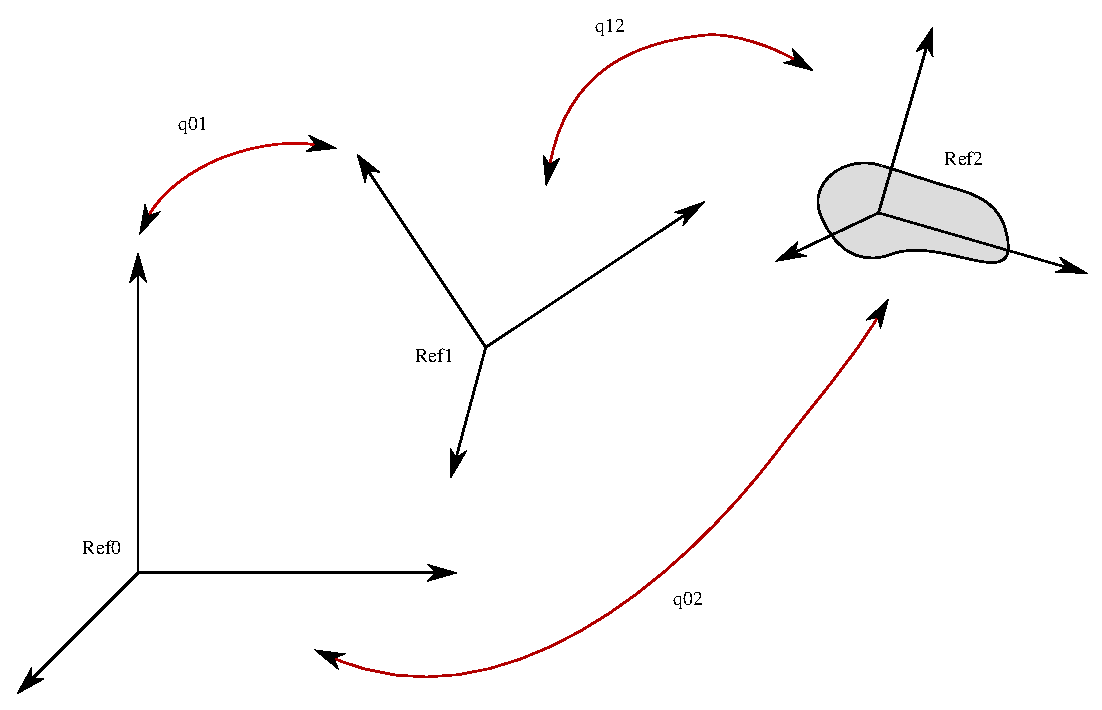
\epsfig{file=figures/SpeedComposition.eps, width=12cm}
\end{center}
%\end{figure}


所以我们可以写为

\begin{equation*}
x^0=q_{01} \o x^1 \o \bar{q}_{01}   \qquad   x^1=q_{12} \o x^2 \o \bar{q}_{12} \qquad    x^0=q_{02} \o x^2 \o \bar{q}_{02}
\end{equation*}

并且替换

\begin{equation*}
x^0=q_{01} \o x^1 \o \bar{q}_{01}  =  q_{01} \o q_{12} \o x^2 \o \bar{q}_{12} \o \bar{q}_{01} 
  =  (q_{01} \o q_{12}) \o x^2 \o (\overline{q_{01} \o q_{12}})
\end{equation*}
  
我们可以确定 $q_{02}$

\begin{equation}
q_{02} = q_{01} \o q_{12}.
\end{equation}

注意 $\omega_{ij}^j = (0,\v{\omega}_{ij}^j)$ 在帧 $j$ 中表示的参考帧 $j$ 相对于帧 $i$ 的旋转速度,并记住 $\omega_{ij}^j = 2\bar{q}_{ij} \o \dot{q}_{ij}$,我们可以写为

\begin{align*}
\omega_{02}^2  &=   2\bar{q}_{02} \o \dot{q}_{02} \\
                              &=   2 (\bar{q}_{12} \o \bar{q}_{01}) \o (\dot{q}_{01} \o q_{12}    +   q_{01} \o \dot{q}_{12}) \\
                              &=   2 \bar{q}_{12} \o \bar{q}_{01} \o \dot{q}_{01} \o q_{12}    +
                                        2 \bar{q}_{12} \o \underbrace{\bar{q}_{01} \o  q_{01}}_{Id} \o \dot{q}_{12} \\
                              &=   \bar{q}_{12} \o \underbrace{(2 \bar{q}_{01} \o \dot{q}_{01})}_{\omega_{01}^1} \o q_{12}    +
                                         \underbrace{2 \bar{q}_{12} \o  \dot{q}_{12}}_{\omega_{12}^2}\\
                              &=  \bar{q}_{12} \o \omega_{01}^1 \o q_{12}    +      \omega_{12}^2 \\
                              &=   \omega_{01}^2   +      \omega_{12}^2.
\end{align*}

也就是说,我们可以添加连续的转速,如果它们表示在同一个参考。\\
在 Cubsat 的情况下, $\v{\omega}_{02}^2$ 是惯性参考模型中以机体坐标表示的卫星的旋转速度 $\v{\omega}'$ ;我们将在这里注意到它 $\v{\omega}'_{Inertial}$ 。另一方面, $\v{\omega}_{12}^2$ 是卫星在非惯性参考模型 (即在轨道参考系中,ORF) 中的旋转速度 $\v{\omega}'$ ;我们会注意到 $\v{\omega}'_{NonInertial}$。 \\
$\v{\omega}_{01}^1$ 是 ORF 中表示的 ORF,即 $\v{\omega}_o$,而 $\v{\omega}_{01}^2$ 是相同的矢量,在机体参考系中变换。这个转换是由非惯性模型 (在上面展开的是 $\bar{q}_{12}$)中的 $R^T$ 执行的。\\
换句话说,我们可以将惯性和非惯性公式(模型)中的 $\v{\omega}'$ 链接在一起

\begin{equation}
\v{\omega}'_{Inertial} = R^T_{NonInertial} \v{\omega}_o + \v{\omega}'_{NonInertial}.
\label{SC_comp}
\end{equation}

这是用来计算非惯性模型动能的速度。




%Bibliographie:
%\begin{thebibliography}{9}

%\bibitem{QFREP}
%	Quaternion, Finite Rotation and Euler Parameters\\
%	Arend L. Schwab \\
%	\emph{http://tam.cornell.edu/\~{}als93/quaternion.pdf}
%	
%\bibitem{Gros}
%	Quaternion based dynamics - Single Turbine Aircraft - Lagrange and Hamiltonian approaches \\
%	S. Gros\\
%	LA, EPFL.
%		
%\bibitem{Gold}
%	Classical Mechanics \\
%	Herbert Goldstein.
%	
%\bibitem{Wells}
%	Lagrangian Dynamics \\
%	Dare A. Wells \\
%	Schaum's Outline Series.
	
	

%	\bibitem{lamport94}
%	  Leslie Lamport,
%	  \emph{\LaTeX: A Document Preparation System}.
%	  Addison Wesley, Massachusetts,
%	  2nd Edition,
%	  1994.

%rajouter: bouquin de Papa (mcanique), bouquin OpenGL	
	
%\end{thebibliography}





%\end{document}

\pagebreak 

\graphicspath{{SubDocuments/Q2E_latex/}}
%\documentclass[11pt]{article}
%\usepackage{geometry}                % See geometry.pdf to learn the layout options. There are lots.
%\geometry{a4paper}                   % ... or a4paper or a5paper or ... 
%\usepackage{graphicx}
%\usepackage{amssymb}
%\usepackage{epstopdf}
%\usepackage{color}
%\DeclareGraphicsRule{.tif}{png}{.png}{`convert #1 `dirname #1`/`basename #1 .tif`.png}

%\title{Euler Angles to Quaternions}
%\author{Basile Graf}
%%\date{}                                           % Activate to display a given date or no date

%\begin{document}
%\maketitle
%%\section{}
%%\subsection{}



\section{欧拉角到四元数}
\label{sec_Eul2Quat}

每个轴绕欧拉角的三个旋转可以被写为 \\

$$ R_{\psi} =  \left[ \begin {array}{ccc} \cos \left( {\it \psi} \right) &-\sin \left( {\it \psi} \right) &0\\\noalign{\medskip}\sin \left( {\it \psi} \right) &\cos \left( {\it \psi} \right) &0\\\noalign{\medskip}0&0&1\end {array} \right] $$\\

$$ R_{\theta} =  \left[ \begin {array}{ccc} \cos \left( {\it \theta} \right) &0&\sin \left( {\it \theta} \right) \\\noalign{\medskip}0&1&0\\\noalign{\medskip}-\sin \left( {\it \theta} \right) &0&\cos \left( {\it \theta} \right) \end {array} \right] $$\\


$$ R_{\phi} =  \left[ \begin {array}{ccc} 1&0&0\\\noalign{\medskip}0&\cos \left( {\it \phi} \right) &-\sin \left( {\it \phi} \right) \\\noalign{\medskip}0&\sin \left( {\it \phi} \right) &\cos \left( {\it \phi} \right) \end {array} \right] $$\\

它们结合在一起定义了旋转矩阵 \\

$$ R = R_{\phi} R_{\theta} R_{\psi}. $$\\ 

这三个旋转也可以表示为四元数旋转 \\

\begin{center}
$ \mathbf{q_{\phi}} =  \left[ \begin {array}{c} \cos \left( \frac{1}{2}\,{\it \phi} \right) \\\noalign{\medskip}\sin \left( \frac{1}{2}\,{\it \phi} \right) \\\noalign{\medskip}0\\\noalign{\medskip}0\end {array} \right] $ $\qquad$ $ \mathbf{q_{\theta}} =  \left[ \begin {array}{c} \cos \left( \frac{1}{2}\,{\it \theta} \right) \\\noalign{\medskip}0\\\noalign{\medskip}\sin \left( \frac{1}{2}\,{\it \theta} \right) \\\noalign{\medskip}0\end {array} \right] $ $\qquad$ $ \mathbf{q_{\psi}} =  \left[ \begin {array}{c} \cos \left( \frac{1}{2}\,{\it \psi} \right) \\\noalign{\medskip}0\\\noalign{\medskip}0\\\noalign{\medskip}\sin \left( \frac{1}{2}\,{\it \psi} \right) \end {array} \right] .$\\
\end{center}

\vspace{0.8cm}
然后把这三个数相乘就可以得到四元数 \\

$$ \mathbf{q} = \mathbf{q_{\phi}} \circ \mathbf{q_{\theta}} \circ \mathbf{q_{\psi}} =  \left[ \begin {array}{c} \cos \left( \frac{1}{2}\,{\it \phi} \right) \cos \left( \frac{1}{2}\,{\it \theta} \right) \cos \left( \frac{1}{2}\,{\it \psi} \right) -\sin \left( \frac{1}{2}\,{\it \phi} \right) \sin \left( \frac{1}{2}\,{\it \theta} \right) \sin \left( \frac{1}{2}\,{\it \psi} \right) \\\noalign{\medskip}\cos \left( \frac{1}{2}\,{\it \psi} \right) \cos \left( \frac{1}{2}\,{\it \theta} \right) \sin \left( \frac{1}{2}\,{\it \phi} \right) +\cos \left( \frac{1}{2}\,{\it \phi} \right) \sin \left( \frac{1}{2}\,{\it \theta} \right) \sin \left( \frac{1}{2}\,{\it \psi} \right) \\\noalign{\medskip}\cos \left( \frac{1}{2}\,{\it \psi} \right) \cos \left( \frac{1}{2}\,{\it \phi} \right) \sin \left( \frac{1}{2}\,{\it \theta} \right) -\cos \left( \frac{1}{2}\,{\it \theta} \right) \sin \left( \frac{1}{2}\,{\it \phi} \right) \sin \left( \frac{1}{2}\,{\it \psi} \right) \\\noalign{\medskip}\cos \left( \frac{1}{2}\,{\it \phi} \right) \cos \left( \frac{1}{2}\,{\it \theta} \right) \sin \left( \frac{1}{2}\,{\it \psi} \right) +\cos \left( \frac{1}{2}\,{\it \psi} \right) \sin \left( \frac{1}{2}\,{\it \phi} \right) \sin \left( \frac{1}{2}\,{\it \theta} \right) \end {array} \right]. $$ \\ 




注意:此结果取决于欧拉角和旋转轴的顺序和选择中使用的约定!参见文档\cite{mathworksQuat}


%\end{document}  


\pagebreak 

\clearpage\end{CJK*}

%Bibliographie:
%\bibliography{bibliography/cubesat_bibliography}

\begin{thebibliography}{9}

\bibitem{QFREP}
	Quaternion, Finite Rotation and Euler Parameters\\
	Arend L. Schwab \\
	\emph{http://tam.cornell.edu/\~{}als93/quaternion.pdf}
	
\bibitem{Gros}
	Quaternion based dynamics - Single Turbine Aircraft - Lagrange and Hamiltonian approaches \\
	S. Gros\\
	LA, EPFL.
		
\bibitem{Gold}
	Classical Mechanics \\
	Herbert Goldstein.
	
\bibitem{Wells}
	Lagrangian Dynamics \\
	Dare A. Wells \\
	Schaum's Outline Series.
	
	
	
\bibitem{mathworksQuat}
	\emph{http://www.mathworks.com/access/helpdesk/help/toolbox/aeroblks/index.html?}\\
         \emph{ /access/helpdesk/help/toolbox/aeroblks/euleranglestoquaternions.html}
	
%\bibitem{Khalil}
%	Nonlinear Systems \\
%	Third Edition \\
%	Hassan K. Khalil \\
%	Prentice Hall.
	
	

%	\bibitem{lamport94}
%	  Leslie Lamport,
%	  \emph{\LaTeX: A Document Preparation System}.
%	  Addison Wesley, Massachusetts,
%	  2nd Edition,
%	  1994.

%rajouter: bouquin de Papa (mÈcanique), bouquin OpenGL	
	
\end{thebibliography}

%\begin{thebibliography}{20}
%
%\bibitem{Khalil}
%	Nonlinear Systems\\
%	Third Edition\\
%	Hassan K. Khalil\\
%	Prentice Hall
%	
%\bibitem{Lovera}
%	Spacecraft attitude control using magnetic actuators \\
%	M. Lovera, A. Astolfi\\
%	\emph{Automatica} 40 (2004) 1405-1414
%	
%	
%\bibitem{Wisniewski}
%	Fully magnetic attitude control for spacecraft subject to gravity gradient\\
%	R. Wi\'{s}niewski, M. Blanke \\
%	\emph{Automatica} 35 1202-1214
%	
%
%\bibitem{CommentsWisniewski}
%	Comments on "Fully magnetic attitude control for spacecraft subject to gravity gradient"\\
%	Christopher J. Damaren \\
%	\emph{Automatica} 38 (2002) 2189
%	
%\bibitem{nCube}
%	Attitude control for the Norwegian student satellite nCube \\
%	Eli Jerpseth $\cancel{\textrm{O}}$verby \\
%	Norwegian University of Science and Technology, Trondheim.
%
%
%\bibitem{QFREP}
%	Quaternion, Finite Rotation and Euler Parameters\\
%	Arend L. Schwab \\
%	\emph{http://tam.cornell.edu/\~{}als93/quaternion.pdf}
%	
%\bibitem{Gros}
%	Quaternion based dynamics - Single Turbine Aircraft - Lagrange and Hamiltonian approaches \\
%	S. Gros\\
%	LA, EPFL.
%		
%\bibitem{Gold}
%	Classical Mechanics \\
%	Herbert Goldstein.
%	
%\bibitem{Wells}
%	Lagrangian Dynamics \\
%	Dare A. Wells \\
%	Schaum's Outline Series.
%	
%	
%\bibitem{disturbances}
%	Phase B.\\
%	Disturbances and Actuators Dimensioning\\
%	Bastien Despont\\
%	(Swisscube internal document)
%	
%\bibitem{Wertz}
%	Spacecraft Attitude Determination and Control\\
%	Ed. by James R, Wertz\\
%	Kluwer Academic Publishers.
%	
%\bibitem{Wertz2}
%	 Space Mission Analysis and Design \\
%	 Third Edition\\
%	 James R. Wertz, Wiley J. Larson \\
%	 1999, Microcosm/Kluwer
%	
%\bibitem{Gruber}
%	M\'{e}canique g\'{e}n\'{e}rale \\
%	Christian Gruber, Willy Benoit \\
%	1998, Presses polythechniques et universitaires romandes (PPUR).
%	
%\bibitem{Slotine}
%	Applied Nonlinear Control \\
%	J,-J. Slotine \\ 
%	1991, Prentice-Hall
%
%%	\bibitem{lamport94}
%%	  Leslie Lamport,
%%	  \emph{\LaTeX: A Document Preparation System}.
%%	  Addison Wesley, Massachusetts,
%%	  2nd Edition,
%%	  1994.
%	
%	
%\end{thebibliography}





\end{document}
